\section{Experimental Setup}
\label{sec:experimentalSetup}

We evaluated our implementation using trace-based simulation on 
accelerometer traces collected by the robotic testbed and human 
subjects, and audio traces collected in various environments.

While our robotic testbed allows us to run 
live experiments, we chose instead to use trace-based simulation for 
several reasons.  First, it
took the robot close to an hour to complete a single experiment.  A
thorough exploration of the configuration space of the various sensing
approaches we consider would have required months of continuous
live experiments.  Moreover, taking fine grain power consumption
measurements while the robot is in motion is not trivial.


\subsection{Trace Collection}

{\bf Robotic accelerometer traces} We collected the traces by having 
the robot perform multiple runs with
a prototype smartphone attached to it back.  The smartphone ran an
application that kept the device always awake and continuously recorded
accelerometer readings for all three axes.  Each run generated a
trace that included timestamps for the start and end of each action
performed by the robot (which we use as the ground truth for our
experiments) and a list of timestamped acceleration readings.

In each run, the robot performed five different actions: standing
idle, walking, sit-to-stand transitions, stand-to-sit transitions, and
headbutts.  We created runs with three different levels of activity.
Runs in groups 1, 2 and 3 spent 90\% , 50\% and 10\% of the time
standing idle, respectively. The reminder of the time was allocated as
follows: 73\% for walking, 24\% for transitions between sitting and
standing, and 3\% for headbutts.  This setup allows us to experiment
with detecting actions that are common, somewhat frequent, and rare.
In total, the robot executed 18 different runs: 9 for group 1, 6
for group 2 and 3 for group 3.  We generated more runs for groups 1
and 2 because of the lower activity levels compared to group 3. To
eliminate bias, the list of actions was generated randomly for each
run, based on the expected probabilities of each action occurring.

{\bf Human accelerometer traces}
In addition, to validate the applicability of our results to human
scenarios, we collected six hours worth of accelerometer traces from
three different individuals while they perform routine daily
activities: morning commute using public transit, working in a retail
store, and working in an office.  Between 20\% and 37\% of each trace
is spent walking.

{\bf Audio traces} 
To explore the applicability of our approach to sensors other than 
the accelerometer, we collected three half-hour audio traces in
different environments: an office, a coffee shop and outdoors.  We
used audio mixing software to add audio events of interest to the
collected traces.  The audio events of interest include music (5\%
of each trace), speech (5\% of each trace), and sirens (2\% of each 
trace).  The events of interest were randomly selected from a library
of audio files.

\subsection{Applications}

\subsubsection{Accelerometer Applications}

We developed three applications that detect activities that the robot
can perform: walking, posture transitions, and headbutts.  
We chose these
actions because they have similar acceleration signatures to human
activities.  A walking robot has a similar acceleration signature as
its human counterpart, though at a lower intensity.  The headbutts are
meant to represent very infrequent human actions such as falling.  We
found that robot stance transitions between the normal and sitting
postures are very similar in their acceleration signature to humans
sitting down and standing up.  In Section~\ref{sec:results} we show
that the energy saving measured in our experiments with the robot
approximate closely the results of experiments conducted on limited
traces collected from human subjects.

{\bf Steps} Counts how many steps the robot takes when it
  walks. It's algorithm is based on the human step detection algorithm
  proposed by Ryan Libby in~\cite{libbyFootstepDetection}. The
  application takes in raw accelerometer readings and applies a
  low-pass filter on the x-axis acceleration. It then searches for
  local maxima in the filtered x-axis acceleration. Local maxima
  between $2.5\:m/s^2$ and $4.5\:m/s^2$ are detected as steps, given
  that no other steps were detected within the last 100 ms.

{\bf Transitions} Detects transitions between sitting and
  standing.  The application monitors changes in acceleration due to
  gravity on the y and z axes to determine the orientation of the
  device. If the z-axis (up-down relative to the dog) acceleration is
  between $9 m/s^2$ and $11 m/s^2$, and the acceleration on the y-axis
  (front-back relative to the dog) is between $-1 m/s^2$ and $1
  m/s^2$, the device is in a horizontal position and the robot is
  assumed to be in a standing posture. Similarly, if the z-axis
  acceleration is between $7.5 m/s^2$ and $9.5 m/s^2$, and the
  acceleration on the y-axis is between $3.5 m/s^2$ and $5.5 m/s^2$,
  the device is in an angled position and the robot is assumed to be
  in a sitting posture. The application detects transitions by looking
  for posture changes.

{\bf Headbutts} Detects a sudden forward head movement.  The
  application monitors the y-axis acceleration and searches for local
  minima between $-3.75\:m/s^2$ and $-6.75\:m/s^2$.

\subsubsection{Audio Applications}

{\bf Siren Detector} Detects sirens originating from
emergency vehicles.  The application applies a 750 Hz high-pass filter 
in order to remove a significant
potion of sounds that aren't sirens.  The data in each window is transformed 
to the frequency domain using a FFT in order to extract the magnitude of the 
dominant frequency and the mean magnitude of all frequency bins.  The ratio
of the dominant frequency magnitude and the mean magnitude is used to determine
if the window contains pitched sounds.  Pitched sounds between 850 Hz and 1800 Hz
that last longer 650 ms are classified as sirens. 

{\bf Music Journal} Creates a list of all the songs heard during the
day using the web services provided by Echoprint.me \hl{cite?}

{\bf Phrase Detection} Detects specific phrases using web services
accessible via the Google Speech API. \hl{cite?}


\subsection{Configurations}

We evaluate the recall and precision of our applications under the following configurations:

\begin{itemize}

\item {\bf Duty Cycling} The applications wake-up at fixed time 
intervals to collect sensor data for 4 seconds and run the event 
detection algorithms.  If an action is detected, the phone is 
kept awake for another 4 seconds, and goes to sleep otherwise. 

\iffalse
\textbf{Duty Cycling} We modified the applications so that they check
sensor readings periodically and then put the phone to sleep.  On
wake-up, the phone is kept awake for 4 seconds in order to collect
sensor data.  If an action is detected, the phone is kept awake for
another 4 second, and goes to sleep otherwise.  This software only
implementation runs on any mobile device and does not require special
hardware support.
\fi

\item {\bf Batching} The applications wake-up at fixed time intervals to receive the batch of sensor data and run the event detection algorithms.

\iffalse
\textbf{Batching} This configuration emulates hardware support
available on the Nexus 5 for collecting and batching accelerometer
readings while the main processor sleeps.  The application wakes up
periodically, reads the batch of sensor readings, runs the detection
algorithm, and goes back to sleep.
\fi

\item {\bf Generic Wake-up Condition} This configuration simulates the Android's built-in significant motion detector.
We constructed simple classifiers to wake up the device and run the applications when significant activity is detected (significant acceleration or sound).

\item {\bf Simple Configurable Classifier} For each of the 
applications, we constructed simple event classifiers to 
wake up the device and run the event detection 
applications.  A more detailed description of the 
classifiers is available in Section~\ref{sec:classifiers}.

\item {\bf Oracle} A hypothetical ideal implementation that only wakes up
when the event of interest occurs.  Such a wake-up condition would
achieve perfect detection precision and recall, with
the lowest possible power consumption. The difference between the
power consumption of this method and the SCC configuration
provides an upper bound on the potential additional benefits of custom
code offloading.
  
\end{itemize}

For each sensing approach and trace, we measured the amount of sleep
and awake time, the total number of wake-up events, and the recall and
precision of the application.  Finally, we used an energy model
derived from measurements of our prototype to estimate
the average power consumption.  For the {\em Duty Cycling} experiments, 
the power model accounts only for the energy
consumption of the Nexus 4.  For {\em Batching} and {\em Generic Wake-up Condition},
the model also includes the cost of the low-power TI MSP430
micro-controller.  Finally, experiments configured to use {\em SCC} include the cost of 
either the TI MSP430 or the TI Stellaris
LM4F120H5QR, depending on the complexity of the algorithms used by the SCC.

\subsection{Simple Configurable Classifiers}
\label{sec:classifiers}

We created a simple classifier for each of the six applications using
the processing algorithms described in section~\ref{sec:sensorDataAlgorithms}. 
Figure~\ref{fig:sccPipelines} illustrates the pipeline nature of each of the 
SCC we constructed.  Generally, the simple classifiers are simplified versions
of the detection algorithms implemented by the applications.  However, specific
phrase detection is a complex process that requires algorithms not implemented
by our sensor node.  As a compromise, the SCC for the phrase detection application
is used to wake-up the device when any speech is detected.

\hl{TODO: add remaining pipelines && make figure more legible}

\begin{figure}[t]
	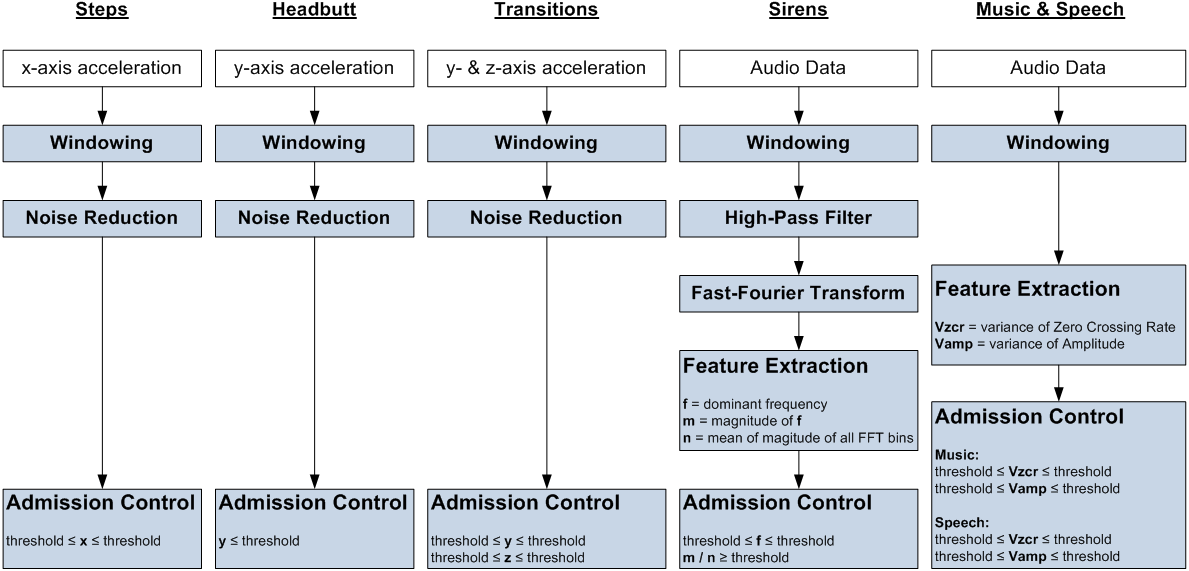
\includegraphics[width=3in]{sccPipelines.png}
	\caption{SCC pipelines for each of the applications.}
	\label{fig:sccPipelines}
\end{figure}



